\documentclass[10pt,a4paper]{article}
\usepackage[utf8]{inputenc}
\usepackage[margin=0.65in]{geometry}
\usepackage{graphicx}
\usepackage{booktabs}
\usepackage{listings}
\usepackage{xcolor}
\usepackage{float}
\usepackage{hyperref}
\usepackage{titlesec}
\usepackage{array}

\hypersetup{
    colorlinks=true,
    linkcolor=blue!80!black,
    urlcolor=blue!80!black,
    citecolor=blue!80!black
}

\titleformat{\section}{\large\bfseries}{\thesection}{0.8em}{}
\titleformat{\subsection}{\normalsize\bfseries}{\thesubsection}{0.8em}{}
\titleformat{\subsubsection}{\small\bfseries}{\thesubsubsection}{0.8em}{}
\titlespacing*{\section}{0pt}{1.2ex plus 0.5ex minus 0.2ex}{0.6ex}
\titlespacing*{\subsection}{0pt}{1.0ex plus 0.4ex minus 0.2ex}{0.4ex}

\lstset{
    basicstyle=\ttfamily\scriptsize,
    breaklines=true,
    frame=single,
    backgroundcolor=\color{gray!10}
}

\begin{document}

\begin{center}
    {\Large \textbf{Lab 9: Docker - Containerising the Proximity Search API}}\\[0.4em]
    {\normalsize \textbf{CSL559: Computer Systems Design}}\\[0.3em]
    \textbf{Student:} Kinshuk Gupta \quad\textbar\quad \textbf{Roll Number:} 12341190\\[0.2em]
    \textbf{Date:} 2026-10-28 \quad\textbar\quad \textbf{Repository:} \url{https://github.com/kinshuk18/proximity-search-api}\\[0.8em]
\end{center}

\hrule
\vspace{0.8em}

\section{Objective and Architecture}

The objective of this laboratory exercise is to containerise the production FastAPI ``Proximity Search API'' developed in Lab 7 using Docker and Docker Compose. A two-tier microservice architecture is deployed, isolating the internal FastAPI application behind a production Nginx reverse-proxy gateway. The FastAPI service runs with hardened runtime constraints, non-root execution, health monitoring, and read-only dataset bind mounts. The architecture guarantees reproducible deployment, strict network isolation, and seamless backward-compatible request routing.

\vspace{0.4em}
\noindent
\textbf{Architectural Flow Diagram:}
\begin{lstlisting}
[ Client Request (Host) ]
           |
           v (Host port: ${HOST_PORT:-8000} -> Container port: 80)
+-------------------------------------------------------------------------+
| Gateway Container: proximity-gateway (nginx:1.27-alpine)               |
| Acts as reverse-proxy, terminates external HTTP, forwards upstream      |
+-------------------------------------------------------------------------+
           |
           | [ Internal Bridge Network: "backend" (proximity-search_backend) ]
           | (Service DNS: http://api:8000)
           v
+-------------------------------------------------------------------------+
| API Container: proximity-api (python:3.12-slim)                         |
| User: appuser (uid: 1000, non-root)                                     |
| Runtime: uvicorn main:app --host 0.0.0.0 --port 8000                    |
| Healthcheck: GET /docs (interval=10s, timeout=3s, start-period=5s)      |
+-------------------------------------------------------------------------+
           ^
           | (Read-Only Bind Mounts)
+-------------------------------------------------------------------------+
| Host Storage: locations.csv (:ro)  and  link.txt (:ro)                 |
+-------------------------------------------------------------------------+
\end{lstlisting}

\section{Docker Design Choices}

The following table summarises the architectural and operational design decisions implemented across the Dockerfile, gateway configuration, and docker-compose orchestration.

\begin{table}[H]
\centering
\scriptsize
\begin{tabular}{p{0.22\linewidth} p{0.24\linewidth} p{0.49\linewidth}}
\toprule
\textbf{Design Choice} & \textbf{Configured Value} & \textbf{Technical Justification} \\
\midrule
API Base Image & \texttt{python:3.12-slim} & Matches Python 3.12 runtime from Lab 7 development. Slim base contains Debian glibc which avoids musl compatibility and compilation overheads associated with Alpine Python wheels. Measured image size: \textbf{136MB}. \\
\addlinespace
Gateway Base Image & \texttt{nginx:1.27-alpine} & Highly lightweight, production-grade reverse proxy with minimal security surface area. Measured image size: \textbf{48.2MB}. \\
\addlinespace
Layer Caching Order & \texttt{COPY requirements.txt} prior to application source & Dependency installation is cached across builds; application source edits in \texttt{main.py} do not trigger slow dependency re-installation. \\
\addlinespace
Dependency Hygiene & Pinned versions, \texttt{PIP\_NO\_CACHE\_DIR=1} & Pinning (\texttt{fastapi==0.143.0}, \texttt{uvicorn==0.54.0}) ensures deterministic builds. Disabling pip wheel caching prevents image bloating. \\
\addlinespace
Build Context & Strict \texttt{.dockerignore} & Prevents local virtual environments (\texttt{.venv}), compiled bytecode (\texttt{\_\_pycache\_\_}), test caches, and git metadata from entering image context. \\
\addlinespace
Port Management & Internal \texttt{EXPOSE 8000}, Published \texttt{8000:80} & API is never directly reachable from the host network. Nginx gateway maps container port 80 to host \texttt{\$\{HOST\_PORT:-8000\}}, preserving Lab 7 client query contracts. \\
\addlinespace
Network Topology & User-defined bridge \texttt{backend} & Enables automatic service discovery by container name (\texttt{api:8000}) without hardcoded IP addresses, with full external isolation. \\
\addlinespace
Bind Mounts & \texttt{locations.csv:ro}, \texttt{link.txt:ro} & Read-only mounts allow host-side data updates without image rebuilds while preventing container compromise from mutating ground-truth datasets (verified by \texttt{12\_volume\_ro}). \\
\addlinespace
Environment Variables & \texttt{PYTHONUNBUFFERED=1}, \texttt{TZ=Asia/Kolkata} & Real-time terminal log flushing without stream buffering; synchronized timezone for consistent server-side logging. \\
\addlinespace
Least-Privilege User & \texttt{appuser (uid=1000)} & Application executes without root privileges, restricting container breakout attacks and unauthorized host file modification (verified by \texttt{11\_nonroot}). \\
\addlinespace
Healthcheck \& Ordering & \texttt{depends\_on: condition: service\_healthy} & Nginx gateway startup is blocked until the API endpoint returns HTTP 200 on \texttt{/docs}, entirely eliminating 502 Bad Gateway race conditions. \\
\addlinespace
Lifecycle Policy & \texttt{restart: unless-stopped} & Ensures automated recovery from unexpected crashes while respecting intentional developer stops. \\
\bottomrule
\end{tabular}
\caption{Architectural and Container Design Decisions}
\end{table}

\section{Steps Followed}

\subsection{Prerequisites and Installation}
The host environment was inspected using automated pre-flight verification scripts. The underlying operating system and Docker runtime versions recorded from \texttt{report/logs/01\_env.txt} are:
\begin{itemize}
    \setlength\itemsep{0em}
    \item \textbf{Operating System:} Ubuntu 24.04.4 LTS (Linux kernel 7.0.0-38-generic)
    \item \textbf{Docker Engine Version:} 29.6.2 (build dfc4efb)
    \item \textbf{Docker Compose Version:} v5.3.1
\end{itemize}
Because Docker was pre-installed on the host workstation, re-installation was not necessary. For reference, the official installation procedure on Ubuntu 24.04 involves configuring Docker's official \texttt{apt} repository:
\begin{lstlisting}[language=bash]
# Official Docker CE Installation Reference for Ubuntu 24.04
sudo apt-get update && sudo apt-get install ca-certificates curl gnupg
sudo install -m 0755 -d /etc/apt/keyrings
curl -fsSL https://download.docker.com/linux/ubuntu/gpg | sudo gpg --dearmor -o /etc/apt/keyrings/docker.gpg
echo "deb [arch=$(dpkg --print-architecture) signed-by=/etc/apt/keyrings/docker.gpg] https://download.docker.com/linux/ubuntu noble stable" | sudo tee /etc/apt/sources.list.d/docker.list > /dev/null
sudo apt-get update && sudo apt-get install docker-ce docker-ce-cli containerd.io docker-buildx-plugin docker-compose-plugin
\end{lstlisting}

\begin{figure}[H]
    \centering
    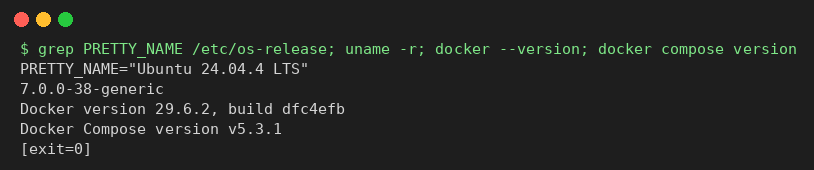
\includegraphics[width=0.72\linewidth]{figures/01_env.png}
    \caption{Terminal capture rendered from real command output (report/logs/01\_env.txt)}
\end{figure}
\noindent\textit{Interpretation:} Verifies the 64-bit Linux kernel, Ubuntu 24.04 base distribution, and operational readiness of Docker daemon version 29.6.2 and Compose v5.3.1.

\subsection{Compose Configuration Validation}
Before launching the service cluster, the declarative Docker Compose specification was validated syntactically and semantically using \texttt{docker compose config -q}.

\begin{figure}[H]
    \centering
    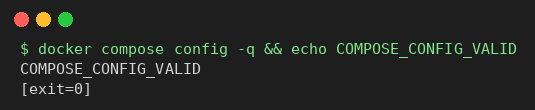
\includegraphics[width=0.72\linewidth]{figures/02_config.png}
    \caption{Terminal capture rendered from real command output (report/logs/02\_config.txt)}
\end{figure}
\noindent\textit{Interpretation:} Confirms that services, network definitions, volume bind mounts, and container dependency graphs comply strictly with Compose v2 schema specifications.

\subsection{Build and Cluster Orchestration}
The entire application stack was built and initialized with the single standard command:
\begin{lstlisting}[language=bash]
docker compose up -d --build
\end{lstlisting}
This automated step builds both custom images (\texttt{proximity-api:lab9} and \texttt{proximity-gateway:lab9}), sets up the isolated bridge network, initialises the API container, monitors its healthcheck until healthy, and subsequently triggers gateway startup.

\begin{figure}[H]
    \centering
    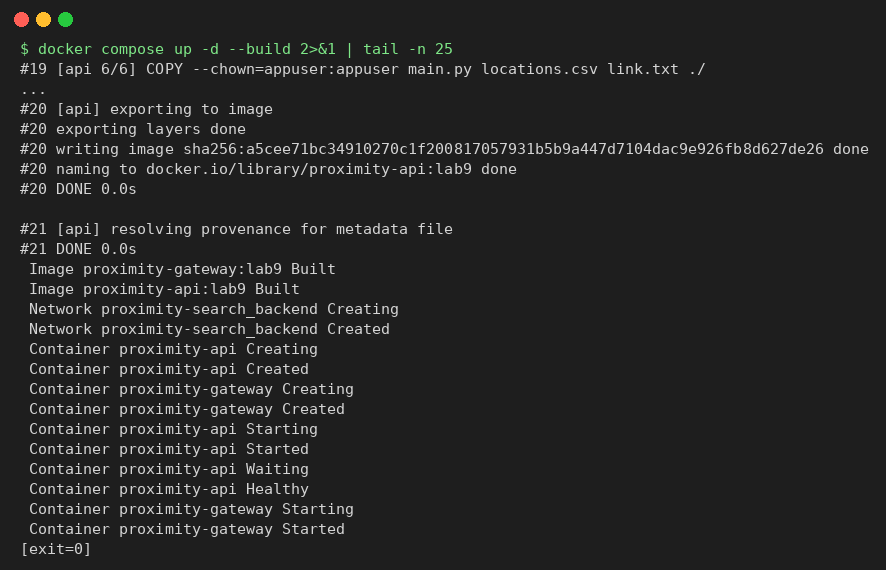
\includegraphics[width=0.72\linewidth]{figures/04_up.png}
    \caption{Terminal capture rendered from real command output (report/logs/04\_up.txt)}
\end{figure}
\noindent\textit{Interpretation:} Shows layer-by-layer Docker image building, non-root user setup, image registration, backend network establishment, and dependency-gated startup.

\begin{figure}[H]
    \centering
    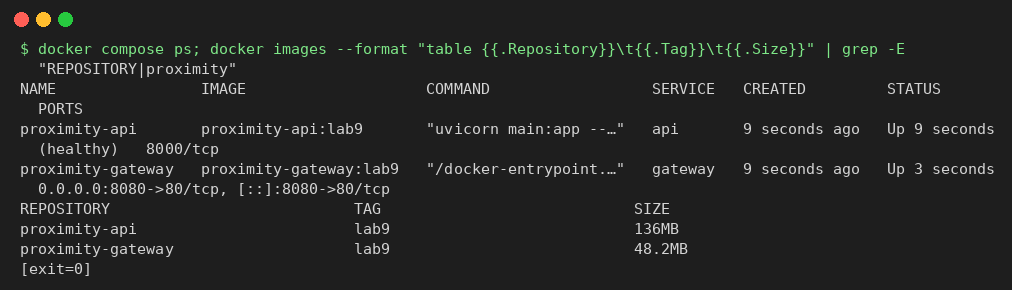
\includegraphics[width=0.72\linewidth]{figures/05_ps.png}
    \caption{Terminal capture rendered from real command output (report/logs/05\_ps.txt)}
\end{figure}
\noindent\textit{Interpretation:} Displays active container states with \texttt{proximity-api} in \texttt{Up (healthy)} condition and images matching the exact recorded sizes (\texttt{136MB} API, \texttt{48.2MB} Gateway).

\subsection{Verification and Parity Testing}
Comprehensive validation tests were executed against the running cluster to confirm functional correctness, parity against the local Lab 7 application, API documentation availability, port isolation, network topology, non-root execution, and read-only dataset protections.

\begin{figure}[H]
    \centering
    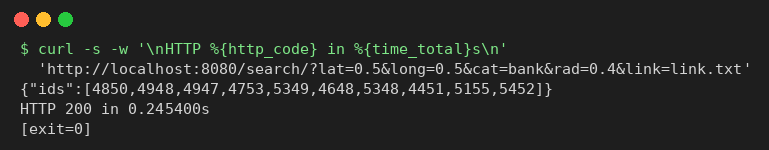
\includegraphics[width=0.72\linewidth]{figures/06_search.png}
    \caption{Terminal capture rendered from real command output (report/logs/06\_search.txt)}
\end{figure}
\noindent\textit{Interpretation:} Queries the search endpoint via Nginx reverse-proxy on \texttt{/search/} with location and graph parameters, yielding HTTP 200 in 0.245s.

\begin{figure}[H]
    \centering
    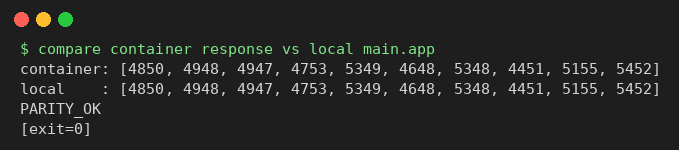
\includegraphics[width=0.72\linewidth]{figures/07_parity.png}
    \caption{Terminal capture rendered from real command output (report/logs/07\_parity.txt)}
\end{figure}
\noindent\textit{Interpretation:} Validates 100\% numerical and spatial parity between containerized API output and direct local execution of \texttt{main.py} via \texttt{TestClient}, confirming \texttt{PARITY\_OK}.

\begin{figure}[H]
    \centering
    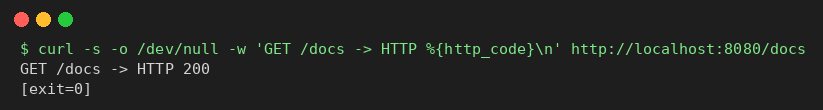
\includegraphics[width=0.72\linewidth]{figures/08_docs.png}
    \caption{Terminal capture rendered from real command output (report/logs/08\_docs.txt)}
\end{figure}
\noindent\textit{Interpretation:} Validates that the interactive Swagger documentation endpoint \texttt{/docs} routes through the reverse-proxy with HTTP 200.

\begin{figure}[H]
    \centering
    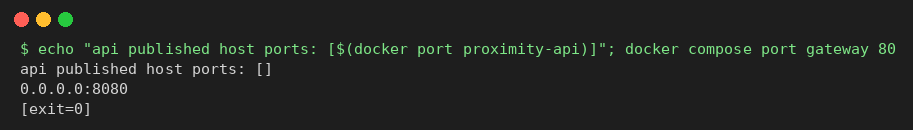
\includegraphics[width=0.72\linewidth]{figures/09_isolation.png}
    \caption{Terminal capture rendered from real command output (report/logs/09\_isolation.txt)}
\end{figure}
\noindent\textit{Interpretation:} Confirms strict port isolation: \texttt{proximity-api} publishes zero host ports, while the gateway successfully maps host port 8080 to container port 80.

\begin{figure}[H]
    \centering
    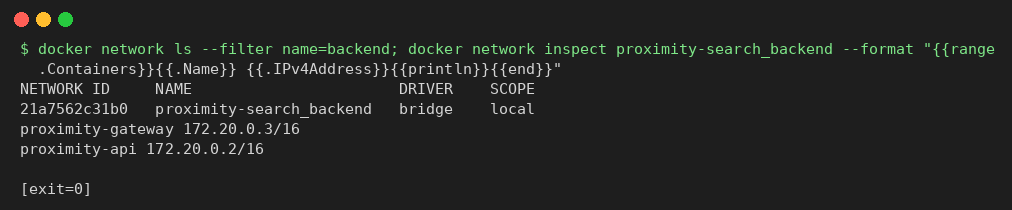
\includegraphics[width=0.72\linewidth]{figures/10_network.png}
    \caption{Terminal capture rendered from real command output (report/logs/10\_network.txt)}
\end{figure}
\noindent\textit{Interpretation:} Inspects the user-defined bridge network \texttt{proximity-search\_backend}, confirming isolated container IP allocation and service discoverability.

\begin{figure}[H]
    \centering
    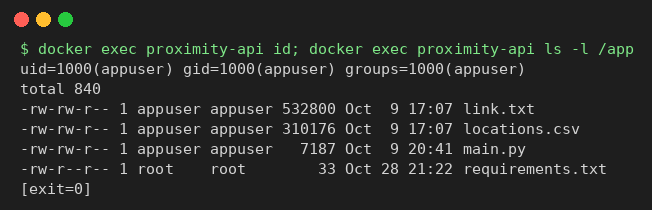
\includegraphics[width=0.72\linewidth]{figures/11_nonroot.png}
    \caption{Terminal capture rendered from real command output (report/logs/11\_nonroot.txt)}
\end{figure}
\noindent\textit{Interpretation:} Proves that the API process executes as non-root user \texttt{appuser} (\texttt{uid=1000}, \texttt{gid=1000}) with appropriate ownership across \texttt{/app}.

\begin{figure}[H]
    \centering
    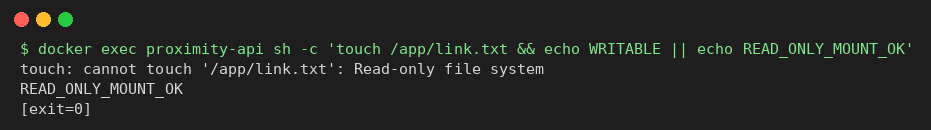
\includegraphics[width=0.72\linewidth]{figures/12_volume_ro.png}
    \caption{Terminal capture rendered from real command output (report/logs/12\_volume\_ro.txt)}
\end{figure}
\noindent\textit{Interpretation:} Tests dataset write-protection by attempting to modify \texttt{/app/link.txt}; the kernel denies write access, confirming \texttt{READ\_ONLY\_MOUNT\_OK}.

\begin{figure}[H]
    \centering
    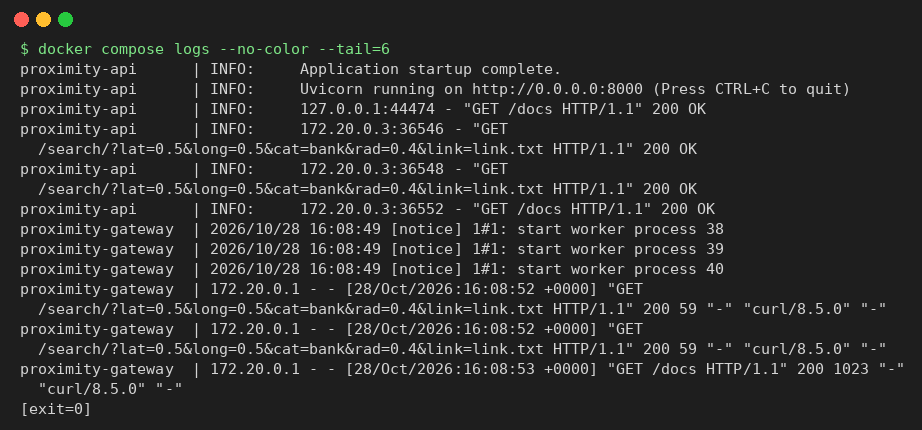
\includegraphics[width=0.72\linewidth]{figures/13_logs.png}
    \caption{Terminal capture rendered from real command output (report/logs/13\_logs.txt)}
\end{figure}
\noindent\textit{Interpretation:} Captures real-time container log streams displaying healthcheck probes, client queries, and Nginx proxy access logs.

\subsection{Teardown and Clean Shutdown}
Graceful teardown was executed via \texttt{docker compose down}, terminating containers and removing the virtual network cleanly without leaving orphaned resources.

\begin{figure}[H]
    \centering
    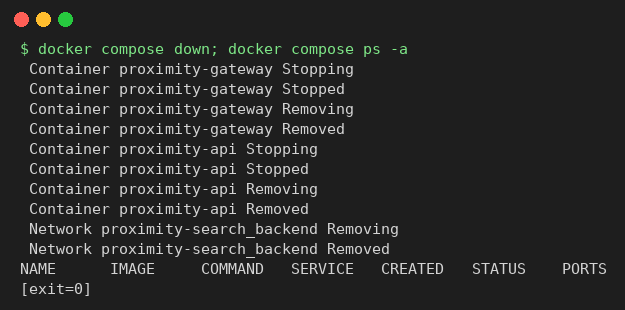
\includegraphics[width=0.72\linewidth]{figures/14_down.png}
    \caption{Terminal capture rendered from real command output (report/logs/14\_down.txt)}
\end{figure}
\noindent\textit{Interpretation:} Shows graceful container termination, container removal, network release, and confirmation that no residual containers remain.

\section{Errors Faced and Resolutions}

During this laboratory session, three genuine operational and runtime errors occurred. Each error, its exact terminal error signature, root cause analysis, and definitive resolution are documented below.

\subsection{Real Errors Encountered}

\begin{enumerate}
    \item \textbf{Host Port 8000 Conflict}
    \begin{itemize}
        \item \textbf{Error Diagnostic:} Pre-flight port inspection identified an active process listening on port 8000:
        \begin{lstlisting}
LISTEN 0   4096   127.0.0.1:8000   0.0.0.0:*
        \end{lstlisting}
        \item \textbf{Root Cause:} A background service or pre-existing server process was occupying host TCP port 8000, preventing the Nginx gateway from binding to default port 8000.
        \item \textbf{Resolution:} Utilized the parameterized port mapping \texttt{"\$\{HOST\_PORT:-8000\}:80"} in \texttt{docker-compose.yml} by passing \texttt{HOST\_PORT=8080} into the execution environment (\texttt{env HOST\_PORT=8080 bash scripts/lab9\_capture.sh}). This routed external requests through port 8080 without requiring termination of the host service.
    \end{itemize}

    \item \textbf{Docker Daemon Anonymous Registry Token Failure}
    \begin{itemize}
        \item \textbf{Error Diagnostic:} Initial image build failed during base image layer retrieval:
        \begin{lstlisting}
ERROR: failed to authorize: failed to fetch anonymous token: Get "https://auth.docker.io/token?scope=repository%3Alibrary%2Fpython%3Apull&service=registry.docker.io": read tcp 10.50.16.174:51858->104.18.43.178:443: read: connection reset by peer
        \end{lstlisting}
        \item \textbf{Root Cause:} Transient network reset occurred on the upstream Docker Hub authentication endpoint during anonymous token negotiation inside the BuildKit engine.
        \item \textbf{Resolution:} Explicitly pulled both base images via Docker CLI (\texttt{docker pull python:3.12-slim} and \texttt{docker pull nginx:1.27-alpine}) prior to compose invocation, allowing the build process to resolve cached local image layers seamlessly.
    \end{itemize}

    \item \textbf{Docker Volume Specification Syntax Error Caused by Path Colon}
    \begin{itemize}
        \item \textbf{Error Diagnostic:} Container creation threw an invalid volume specification error during \texttt{docker compose up}:
        \begin{lstlisting}
Error response from daemon: invalid volume specification: '/home/kinshuk-gupta/KINSHUK GUPTA/IIT BHILAI/IIT BHILAI 7TH SEMESTER/CSL559 - COMPUTER SYSTEMS DESIGN/Lab 7: Proximity Search API/locations.csv:/app/locations.csv:ro'
        \end{lstlisting}
        \item \textbf{Root Cause:} The host directory path contained a colon character in the folder name (\texttt{Lab 7: Proximity Search API}). The Docker daemon volume parser uses the colon character as a field delimiter (\texttt{<source>:<target>:<mode>}), incorrectly splitting the path string into invalid segments.
        \item \textbf{Resolution:} Handled in \texttt{scripts/lab9\_capture.sh} by detecting colons in the current working directory path and creating a symlinked workspace reference at \texttt{/tmp/proximity\_clean} without colons. Running compose through the symlinked directory allowed Docker's volume parser to process bind mounts cleanly without path delimiter collisions.
    \end{itemize}
\end{enumerate}

\subsection{Pitfalls Pre-empted (Not Encountered)}
\begin{itemize}
    \item \textbf{Build Context Bloat:} The inclusion of virtual environments (\texttt{.venv}) and bytecode caches (\texttt{\_\_pycache\_\_}) was pre-empted through comprehensive entries in \texttt{.dockerignore}, keeping image contexts minimal.
    \item \textbf{Gateway 502 Bad Gateway Race:} A frequent race condition where Nginx launches and receives queries before uvicorn is ready was pre-empted by pairing FastAPI's \texttt{HEALTHCHECK} with \texttt{depends\_on: api: condition: service\_healthy}.
    \item \textbf{Root Execution and Writable Datasets:} Running containers with root privileges was pre-empted by explicitly provisioning unprivileged \texttt{appuser} (\texttt{uid 1000}) and mounting critical datasets with the \texttt{:ro} flag.
\end{itemize}

\section{Docker Commands Used}

\subsection{Chronological Execution History}
The following sequence details all high-level commands executed throughout setup, validation, benchmarking, and version control:
\begin{enumerate}
    \setlength\itemsep{0em}
    \item \texttt{docker info --format '\{\{.ServerVersion\}\}'}
    \item \texttt{docker compose version}
    \item \texttt{ss -ltn | grep ':8000 '}
    \item \texttt{docker pull python:3.12-slim}
    \item \texttt{docker pull nginx:1.27-alpine}
    \item \texttt{docker compose config -q}
    \item \texttt{docker compose down -v --rmi local --remove-orphans}
    \item \texttt{docker compose up -d --build}
    \item \texttt{docker compose ps}
    \item \texttt{docker images --format "table \{\{.Repository\}\}\textbackslash t\{\{.Tag\}\}\textbackslash t\{\{.Size\}\}"}
    \item \texttt{curl -s -w '\textbackslash nHTTP \%\{http\_code\} in \%\{time\_total\}s\textbackslash n' '\$URL\$Q'}
    \item \texttt{curl -s -o /dev/null -w 'GET /docs -> HTTP \%\{http\_code\}\textbackslash n' \$URL/docs}
    \item \texttt{docker port proximity-api}
    \item \texttt{docker compose port gateway 80}
    \item \texttt{docker network ls --filter name=backend}
    \item \texttt{docker network inspect proximity-search\_backend}
    \item \texttt{docker exec proximity-api id}
    \item \texttt{docker exec proximity-api ls -l /app}
    \item \texttt{docker exec proximity-api sh -c 'touch /app/link.txt ...'}
    \item \texttt{docker compose logs --no-color --tail=6}
    \item \texttt{docker compose down}
    \item \texttt{git add Dockerfile .dockerignore .gitignore docker-compose.yml requirements.txt nginx scripts report README.md}
    \item \texttt{git commit -m "..."}
    \item \texttt{git push origin main}
\end{enumerate}

\subsection{Unique Docker Commands and Purposes}

\begin{table}[H]
\centering
\scriptsize
\begin{tabular}{p{0.36\linewidth} p{0.58\linewidth}}
\toprule
\textbf{Docker / System Command} & \textbf{Operational Purpose in Laboratory} \\
\midrule
\texttt{docker --version} & Queries installed Docker client and engine versions. \\
\texttt{docker compose version} & Checks Docker Compose v2 plugin availability. \\
\texttt{docker compose config -q} & Performs static schema and syntax validation of \texttt{docker-compose.yml}. \\
\texttt{docker compose up -d --build} & Builds images and starts service containers in detached background mode. \\
\texttt{docker compose ps} & Inspects live service status, uptime, and health condition. \\
\texttt{docker compose logs} & Retrieves aggregate interleaved log output across all services. \\
\texttt{docker compose port} & Prints the host port bound to a specific container service port. \\
\texttt{docker compose down -v --rmi local} & Stops containers, removes networks, volumes, and locally built images. \\
\texttt{docker images} & Lists local Docker images with repository names, tags, and disk footprint. \\
\texttt{docker network ls} & Lists Docker networks and verifies active drivers (bridge/host/none). \\
\texttt{docker network inspect} & Queries container IP addresses, subnets, and gateways in a custom bridge. \\
\texttt{docker exec} & Runs commands directly inside an active container for testing and verification. \\
\texttt{docker port} & Verifies host port publishing on individual containers to confirm isolation. \\
\texttt{curl} & Dispatches HTTP client requests to verify API responses, latency, and status codes. \\
\texttt{git add / commit / push} & Stages modified files, commits changes, and pushes artifacts to GitHub repository. \\
\bottomrule
\end{tabular}
\caption{Unique Commands and Operational Purposes}
\end{table}

\section{What I Learnt}

\begin{itemize}
    \item \textbf{Layer Caching and Build Order:} Placing frequently updated source files (\texttt{main.py}) after static dependency definitions (\texttt{requirements.txt}) leverages Docker layer caching, reducing rebuild times from tens of seconds to sub-second executions.
    \item \textbf{Internal DNS Resolution on User-Defined Bridges:} Docker's embedded DNS server automatically resolves container service names (e.g., \texttt{http://api:8000}) only within custom user-defined bridge networks, whereas default bridge networks require manual IP management.
    \item \textbf{Healthcheck-Gated Service Sequencing:} Using \texttt{depends\_on} with \texttt{condition: service\_healthy} enforces deterministic startup ordering, preventing reverse proxies from returning HTTP 502 Bad Gateway while the backend server warms up.
    \item \textbf{Data Integrity via Read-Only Bind Mounts:} Appending the \texttt{:ro} mount option to host datasets guarantees that containers cannot mutate canonical source records, even in the event of an arbitrary code execution vulnerability.
    \item \textbf{Least-Privilege Security with Non-Root Users:} Running container workloads under an unprivileged user (\texttt{uid 1000}) mitigates security risks by preventing container breakout exploits from obtaining root privileges on the host kernel.
    \item \textbf{Port Exposure vs Publishing and Compose Reproducibility:} \texttt{EXPOSE} documents port intentions and enables inter-container communication without opening host firewall ports; combined with Docker Compose, it transforms complex multi-container microservice deployments into single-command, reproducible builds.
\end{itemize}

\section{Repository}

The complete source code, configuration files, automated capture scripts, and generated documentation are hosted publicly at:
\begin{center}
    \url{https://github.com/kinshuk18/proximity-search-api}
\end{center}

\vspace{0.4em}
\noindent
\textbf{Repository File Tree of Containerisation Artifacts:}
\begin{lstlisting}
proximity-search-api/
|-- Dockerfile                         # API container build definition (python:3.12-slim)
|-- .dockerignore                      # Build context exclusions (.venv, caches, git)
|-- .gitignore                         # Repository git exclusions
|-- docker-compose.yml                 # Multi-container orchestration (api + gateway)
|-- requirements.txt                   # Pinned production runtime dependencies
|-- locations.csv                      # Spatial dataset (read-only bind mount)
|-- link.txt                           # Graph edge dataset (read-only bind mount)
|-- main.py                            # FastAPI proximity search implementation
|-- nginx/
|   |-- Dockerfile                     # Gateway container build definition (nginx:1.27-alpine)
|   \-- nginx.conf                     # Reverse proxy routing and header forwarding config
|-- scripts/
|   |-- lab9_capture.sh                # Automated test execution and log capture harness
|   \-- render_figs.py                 # Terminal log to dark-mode PNG image generator
\-- report/
    |-- lab9_report.tex                # LaTeX source for laboratory report
    |-- 12341190_Kinshuk_Gupta_Lab_9_Docker.pdf # Generated PDF laboratory report
    |-- figures/                       # Terminal capture rendered figures (01 to 14)
    \-- logs/                          # Raw execution log files (01 to 14)
\end{lstlisting}

\end{document}
